\begin{figure}[H]%
		\ThisCenterWallPaper{1}{images/\texorpdfstring{\chaptername\thechapter}}%
		\captionlistentry[figure]{Icon of \chaptername\ \thechapter}% figure with chapter and section number
		%\addcontentsline{lof}{figure}{Icon of \chaptername\ \thechapter}% figure without chapter and section number
		\label{fig:\chaptername\thechapter}%
\end{figure}

\vspace*{-3.45cm}
\epigraph{"Begin at the beginning," - the King said, gravely - "and go on till you come to the end; then stop."}{\textit{--- Lewis Carroll}, Alice in Wonderland}

\noindent \large{\textbf{This {\MakeLowercase{\chaptername}}'s contents:}}
\vspace*{-0.65cm}
\minitoc \mtcskip \minilof
\vspace*{-1cm}
\section{Overview} \label{section:Introduction/Overview}
The end of the last century saw the birth of the web.
It was one of most disruptive technological events (since maybe the invention of the transistor or the \acrshort{TCP}/\acrshort{IP} protocol) that radically changed the way people communicate, express and relate to each other.
\begin{quoting}[
	begintext={},
	endtext={\sfcite{WiredArticleWeAretheWeb2005}}
]
	\textit{
		"Although Nelson was polite, charming, and smooth, I was too slow for his fast talk. But I got an aha! from his marvelous notion of hypertext. He was certain that every document in the world should be a footnote to some other document, and computers could make the links between them visible and permanent. But that was just the beginning! Scribbling on index cards, he sketched out complicated notions of transferring authorship back to creators and tracking payments as readers hopped along networks of documents, what he called the docuverse. He spoke of “transclusion” and “intertwingularity” as he described the grand utopian benefits of his embedded structure. It was going to save the world from stupidity."
	}
\end{quoting}
Apart from that last line, today, the web (and the internet in general) has made it possible to have highly interconnected communication, \glspl{transaction} and data transfer in general.
Everyday online is produced and exchanged a gigantic amount of information, data.\sfcite{Marx2013}
The need to store, manage, transfer and efficiently analyze this information is more present than ever today.
\medskip

In addition, the study of networks has brought significant advances to the understanding of complex systems.
Graphs, extremely useful in representing a wide variety of networks, and graph analysis have become crucial to understand the features of these systems.

\begin{figure}[H]%
	\centering%
	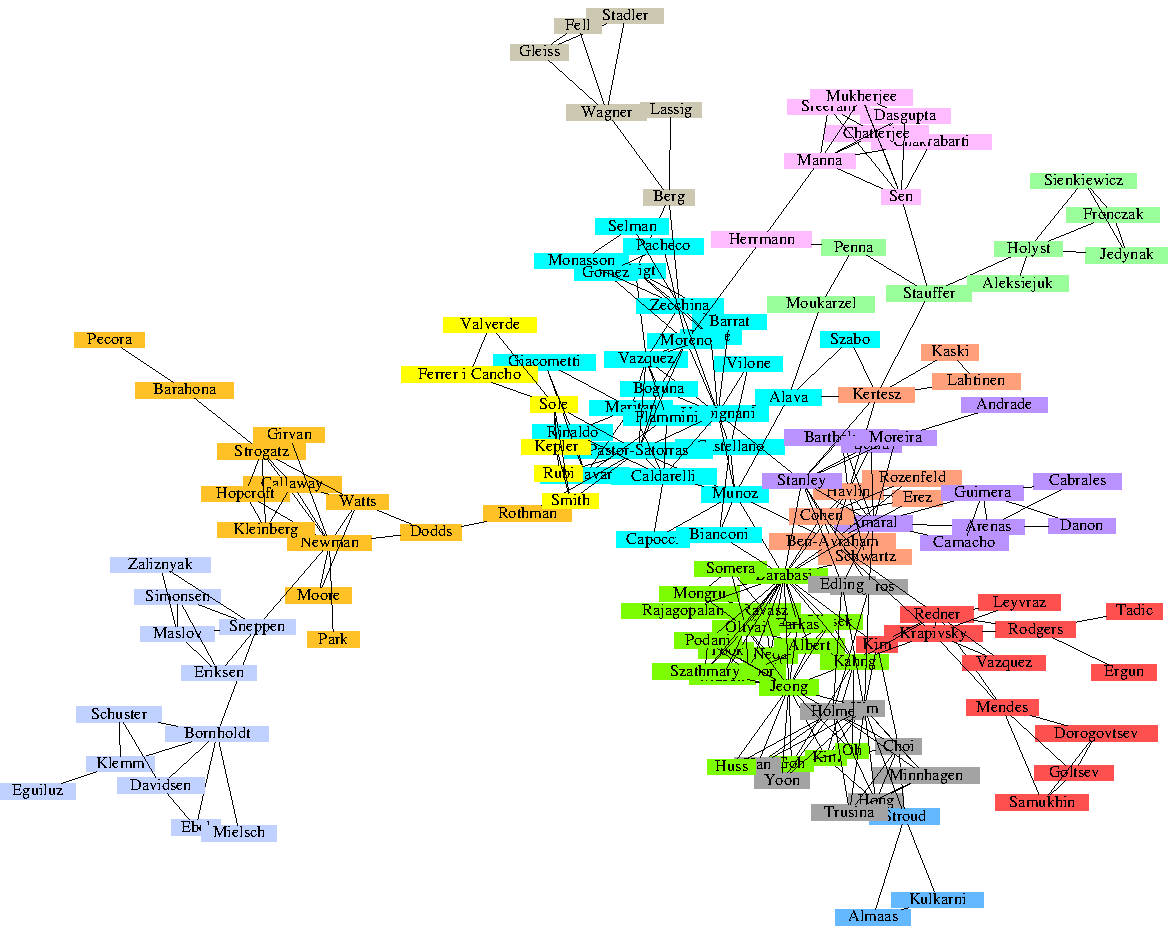
\includegraphics[width=1\textwidth-4pt,%
		bgcolor=white,%
		cfbox=lightestgray % color
			  2pt % rule width
			  0pt % rule separation
			  0pt % margin
	]{images/chapter1/NewmanGirvan2004page12.pdf}%
	\caption[Illustration of the community structure of a network of coauthorships between physicists, scientists]{Illustration of the community structure of a network of coauthorships between physicists, scientists, taken from \citetitle{NewmanGirvan2004} - \citeauthor{NewmanGirvan2004} (\citeyear{NewmanGirvan2004})\sfcite{NewmanGirvan2004}}%
	\label{fig:NewmanGirvan2004page12}%
\end{figure}%
Community structure\sfcite{NewmanGirvan2004}, or clustering is one of the most relevant features of graphs representing real systems.
Individuating such organization structure, detecting communities - is of great importance in various disciplines like:
\setlist{nolistsep} \begin{itemize}[noitemsep]
	\item biology\sfcite{GirvanNewman2002},
	\item sociology\sfcite{ParthasarathyShahZaman2019}, 
	\item computer science
	\item and many more.\sfcite{PallaDerenyiFarkasVicsek2005}
\end{itemize}
  
The nature of the problem makes it hard to solve.
Despite the huge academic effort, it is not yet satisfactorily solved.\sfcite{Fortunato2010}

\section{Focus of the thesis} \label{section:Introduction/Focusofthethesis}
In this thesis shall be performed a practical analysis of large interconnected data representable by graphs (in the mathematical sense of vertices linked by edges) to the end of detecting communities, clusters of more densely connected nodes than others.
For the storage and management of the data \Glspl{graph database} are used.
By making use of \Glspl{graph database} and the advantages they offer in performing complex computations on graphs, with a hands-on approach - clusters (collaboration communities) shall be detected in a graph built on data from a dataset of academic researcher publications.
The dataset used is obtained from \gls{dblp.org}\sfcite{Dagstuhl2021}.

Using a graph database management system, a Label Propagation Community Detection algorithm shall be executed on the graph, thus detecting its clusters and by implementing a \gls{Web Application}, the results of the detection shall be shown to the user whenever queried.

\section{Context} \label{section:Introduction/Context}
The work for this thesis comes, on one hand, in a moment when NoSQL databases have peaked their hype cycle for some time now.
It has been more than a decade now the time graph database management systems started getting developed and used.
These softwares have now been tested in real environments with production data and processes.
They may thus be defined mature enough.

Moreover, the cost for developers, researchers, students to explore this new world and make use of it for their needs - is almost zero.
Community and Educational Editions of the softwares of graph DBMSs are in most cases free and/or open source, with almost all features and license permissions to use in complex projects.

On the other hand, the nowdays higher interconnectivity between people - be it because of faster transportation means, networking infrastructure, online social networks, instant messaging or just easier access and distribution of information - has made it possible to develop software in pairs remotely, write collaboratively, meet (in the sense of work meetings) online or at the nearby coffeeshop with fiber speed internet connection.

\begin{figure}[H]%
	\centering%
	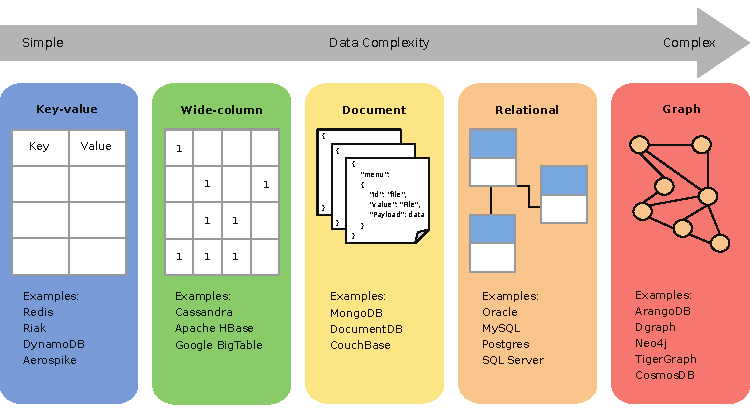
\includegraphics[width=1\textwidth]{%
		images/chapter1/BechbergerPerryman2020page8.pdf%
	}%
	\caption[Database engine types ordered by data complexity]{Database engine types ordered by data complexity, taken from \citetitle{BechbergerPerryman2020} - \citeauthor{BechbergerPerryman2020} (\citeyear{BechbergerPerryman2020})\sfcite{BechbergerPerryman2020}}%
	\label{fig:BechbergerPerryman2020page8}%
\end{figure}%

It probably is more easy today (in the general sense of these years, non-pandemic years) to take a plane, book a hotel, participate in a conference on the other side of the continent and come back with tons of new ideas, new people met and new relations instaurated.
This ease of collaboration makes it possible for newer, larger and geographically more dispersed scientific collaboration communities to flourish.

In this context, capturing a snapshot of who collaborates with whom, which researchers work in smaller groups and which in wider collaboration communities - might be an intriguing exercise to do. Furthermore, as one of the most elegant features of graphs is the possibility to express them graphically in very fancy and expressive diagrams - it would be a huge plus if it was possible to implement an application that displayed the results of the detected clusters.
So, besides detecting the communities, a \gls{WebApp} shall be developed to display the results of the communities in response to user queries.

\subsection{What is known} \label{subsection:Introduction/Context/Whatisknown}
This study is based on two relatively heterogeneous macrotopics, the graph theory, graph databases and the community detection algorithm on one hand - and the development of a \gls{FullStack} \gls{Web Application} involving an \acrshort{API} and a client interface where graphs are rendered on the other hand.

Specifically, it is based on:
\setlist{nolistsep} \begin{itemize}[noitemsep]
	\item graphs
		\setlist{nolistsep} \begin{itemize}[noitemsep]
			\item graph theory literature\sfcite{Bollobas1998}
			\item graph databases literature
				\sfcite{BechbergerPerryman2020,
						BestaPeterGerstenbergerFischerPodstawskiBarthelsAlonsoHoefler2019}
			\item community detection literature from a theoretical point of view
				\sfcite{FortunatoCastellano2007,
						LancichinettiFortunato2009,
						DaoBothorelLenca2020,
						Newman2004,OrmanLabatut2009,
						RosvallDelvenneSchaubLambiotte2019,
						BrandesGaertlerWagner2003,
						LiuChengZhang2019}
				and in practical case studies
				\sfcite{ShaiStanleyGranellTaylorMucha2017,
						WuWuChenLiZhang2021}
			\item \gls{Google}'s \gls{Pregel} algorithm\sfcite{YanChengXingLuNgBu2014} and ArangoDB's custom \gls{Pregel} implementation \sfcite{ArangoDBCommunityDetectionPregel2021}
		\end{itemize}
	\item and general web development
		\setlist{nolistsep} \begin{itemize}[noitemsep]
			\item JavaScript books and documentation
			\item NodeJS books and documentation
			\item ArangoDB documentation
			\item React books and documentation
			\item TypeScript books and documentation
			\item \gls{Cytoscape.JS}\sfcite{CytoscapeJS2021} documentation
		\end{itemize}
\end{itemize}
 
\begin{figure}[H]%
	\centering%
	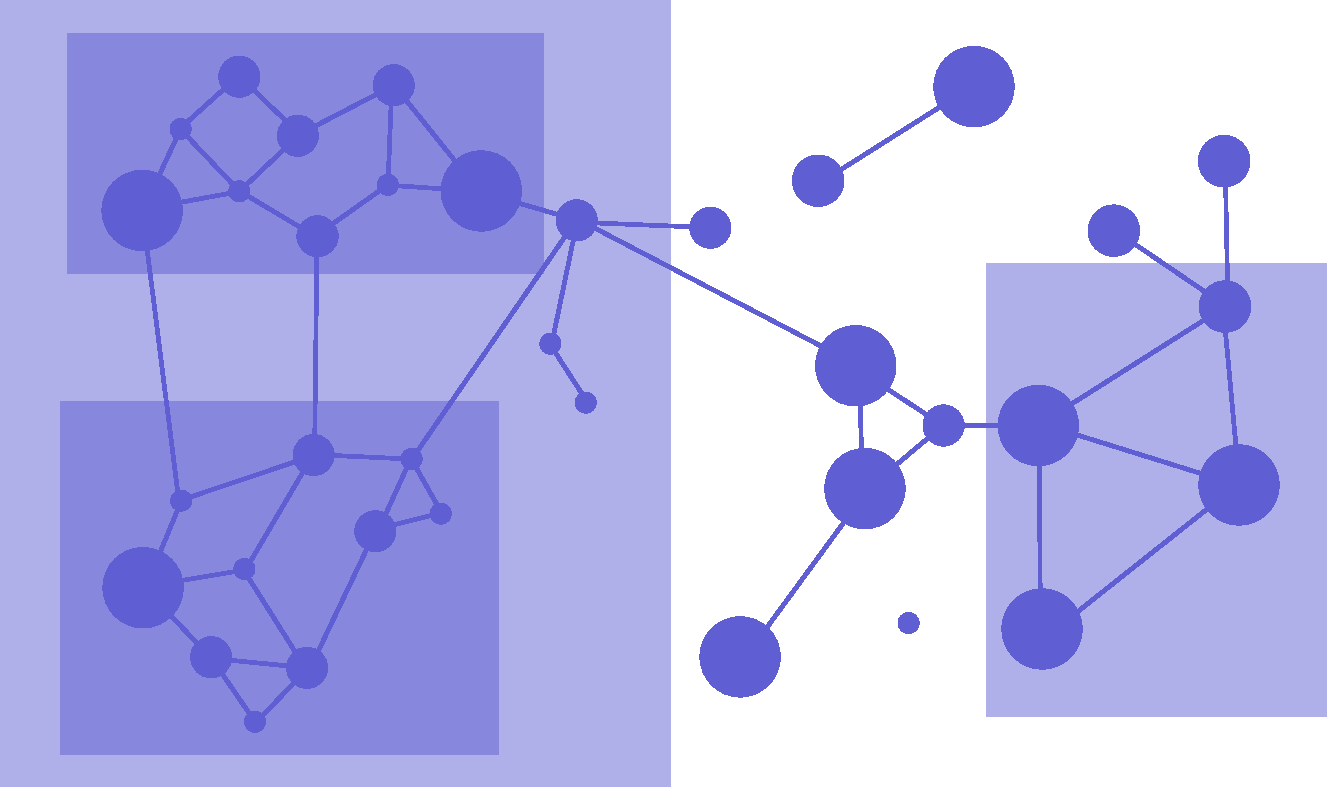
\includegraphics[width=1\textwidth]{images/chapter1/CytoscapeJSCoseBilkent.pdf}%
	\caption[Example of a graph containing compound nodes rendered with CytoscapeJS using Cose Bilkent Layout]{Example of a graph containing compound nodes rendered with \gls{Cytoscape.JS}\sfcite{CytoscapeJS2021} using Cose Bilkent Layout}%
	\label{fig:CytoscapeJSCoseBilkent}%
\end{figure}%

\subsection{Boundaries of the study} \label{subsection:Introduction/Context/Boundariesofthestudy}
This study is limited to the contours of a practical label propagation community detection algorithm execution on the \gls{dblp.org}\sfcite{Dagstuhl2021} dataset of computer science researcher's publications and on the display of the clustering results in a \gls{Web Application}.
No empirical analysis or comparison is made on the efficiency of the algorithm.
No security enforcement mechanisms are implemented in the \gls{Web Application}.
The whole work is kind of a proof-of-concept of what can be done having access to a dataset of interconnected data, a good graph database management system with different graph algorithms offered, libraries to beautifully present the results and lots of imagination.

\subsection{Past similar studies} \label{subsection:Introduction/Context/Pastsimilarstudies}
The problem of detecting communities in scientific collaboration networks has been studied thoroughly for many decades now.
Initially patterns of bibliographic reference relations, like citations, were studied.\sfcite{Price1965}
In recent years, because of advances in information technology and the massive digitalization of documents, data collection and mining capabilities allow for system-level analysis of huge bibliometric datasets that are regularly collected in digital format.
For the first time the structure of scientific collaboration networks was researched.\sfcite{Newman2001structure, Newman200108, Newman200106,
				   NewmanGirvan2004, ChenRedner2010, RadicchiFortunatoVespignani2012}

These studies along with some other specifically related to graph databases and community detection\sfcite{BeisPapadopoulosKompatsiaris2015} are the starting point for the work on this thesis.

\section{Relevance} \label{section:Introduction/Relevance}
Bibliographic databases constitute the most important point for any empirical analysis of
the dynamics involved in scientific activities, citation patterns and in defining the importance of specific contributions, journals, researchers.

There are a variety of compelling reasons for studying the community structure in complex networks.
The partitioning of acquaintances into clusters in social networks represents valuable inflormation of human interactions.
Community structure in metabolic networks helps detect reaction modules.
Communities in the web reveal connections to and from web pages, on related topics.
The underlying scientific community structure in citation networks helps understand both obvious and more subtle relations between groups, subfields, publication entities as well as
the birth or death of subfields or communities.\sfcite{ChenRedner2010}

\paragraph{Benefits of this study}\mbox{}\\\indent
By conducting this work, a step-by-step A to Z description of the of all the implementation process is given.
As a result of this study, it is possible to easily get insights on the collaboration communities in the CS academia, their members and the interactions between them.
\par

\section{Aim and objectives} \label{section:Introduction/Aimandobjectives}
The goals of the work on this thesis are:
\setlist{nolistsep} \begin{itemize}[noitemsep]
	\item usage of a graph database system with a large dataset of real data, specifically computer science academic publications from \gls{dblp.org}\sfcite{Dagstuhl2021};
	\item application of a complex graph algorithm such as the \gls{Pregel} \gls{Label Propagation} Community Detection algorithm
	\item and therefore detection of collaboration clusters of the researchers on that dataset;
	\item implementation of a fullstack \gls{Web Application} to display the results of the detected communities.
\end{itemize}

\subsection{What is developed and why} \label{subsection:Introduction/Aimandobjectives/Whatisexplored}
Different pieces of code are written during the work on this thesis.
Development in the sense of programming, with reasons why, was done on:
\setlist{nolistsep} \begin{itemize}[noitemsep]
	\item \gls{Python} scripts to split and convert XML dataset file to ArangoDB importable JSON files;
	\item Bash scripts to import the data into ArangoDB graph database;
	\item \acrshort{AQL} queries to manipulate the data and transform it to be used as vertices and edges in a graph;
	\item Fullstack self-hosted \gls{Web Application} development made of:
		\setlist{nolistsep} \begin{itemize}[noitemsep]
			\item NodeJS, \gls{Express} and \gls{Apollo Server} backend to serve a \gls{GraphQL} \acrshort{API};
			\item React, Typescript and \gls{Apollo Client} frontend interface to display \gls{Cytoscape} graphs of the detected communities.
		\end{itemize}
	\item \LaTeX\ and Beamer functions used in writing this thesis and the presentation.
\end{itemize}

\subsection{What is determined} \label{subsection:Introduction/Aimandobjectives/Whatisdetermined}
As stated in \hyperref[section:Introduction/Aimandobjectives]{\S\ \ref{section:Introduction/Aimandobjectives} - \nameref{section:Introduction/Aimandobjectives}}, one of the objectives of this work is to determine the collaboration communities between academic researchers in the field of computer science.
For each of the entities involved, like authors, publications, editors, publishers, a community of which they are part of - is determined.
The same is done with affiliation institutions, schools, journal and series.

\subsection{The process} \label{subsection:Introduction/Aimandobjectives/How}
The work for this thesis is divided in three distinct macroparts, with many iterations between them (not to be confused with the parts into which this document is organized):
\setlist{nolistsep} \begin{enumerate}[noitemsep]
	\item The first part of the work is on getting familiarized with the different topics involved.
    So, a profound literature review is conducted.
	\item The second part is about getting the hands dirty with graph databases, using them with the chosen dataset and applying the selected cluster detection algorithm to find the communities.
	\item The third and last part involves the development of the \gls{Web Application} to display the results of the second part with fancy graphs in a user friendly interface.
\end{enumerate}

\section{Contributions in this thesis} \label{section:Introduction/Contributionsinthisthesis}
While the work on this thesis is built on the math concepts of graph theory (commonly known as a difficult subject for students) and on relatively new technologies in computer science such as graph databases and \gls{GraphQL}, React (for web app development) - its advancements of the scientific knowledge are humble.
It might be considered to be a new footprint, a new trail, open for more in-depth future works.

It is shown how new information was produced from the application of a community detection algorithm on data of CS academic researchers.
Furthermore it is shown how it is possible to visually express the clustering results using beautiful graphs embedded in the implemented \gls{WebApp}.

This whole project is a nice practical exercise and might also be a good starting point for other future studies.

\section{Document layout} \label{section:Introduction/Documentlayout}
The document is divided into two parts.
The first part is about a literature review of graph theory, graph databases and algorithms, including the process of detecting the communities.
The second part of the thesis is about the implementation of a \gls{Web Application} with graph databases, \gls{GraphQL} \acrshort{API} and graph rendering libraries in order to display the results of the detected communities.
\medskip

In \hyperref[Preface]{\S\ \ref{Preface} - \nameref{Preface}} is given some general information on the thesis, what it covers, indications on how to get and run the code, description of the notations used, a word on cover and chapter illustrations, a graph of how is best or possible to read the chapters of the document and some basic statistics on the numbers of the document.

Follows some brief information on the author.
\medskip

\textbf{Part I} is composed of the following chapters:

In \hyperref[chapter:Introduction]{\S\ \ref{chapter:Introduction} - \nameref{chapter:Introduction}} (this chapter) a general introduction to the subject is presented.
Firstly the focus of the thesis is stated, with the relative context and relevance.
Then aim and objectives of the thesis are described, followed by the contributions of the work and finally this general layout of the document.

In \hyperref[chapter:LiteratureReview]{\S\ \ref{chapter:LiteratureReview} - \nameref{chapter:LiteratureReview}} an overview or the current state of knowledge is presented.
Firstly a brief review of Graph Theory concepts and algorithms are reported.
Afterwards, Graph Database Systems and Querying Languages are considered, closing the chapter with a comparison between them.

In \hyperref[chapter:CommunityDetection]{\S\ \ref{chapter:CommunityDetection} - \nameref{chapter:CommunityDetection}} an in depth review of the community detection methodologies is presented. The chosen algorithm is described, its execution is brought and some preliminary results are shown.
\medskip

\textbf{Part II}'s layout is the following:

In \hyperref[chapter:ImplementingtheWebApp]{\S\ \ref{chapter:ImplementingtheWebApp} - \nameref{chapter:ImplementingtheWebApp}} initially the hardware and OS used is described.
Then the data preparation, importing and manipulation is presented.
Follows the \gls{GraphQL} \acrshort{API} implementation and the frontend UI interface afterwards.
Closing the chapter are the updates made after the clusters were detected.

In \hyperref[chapter:Displayoftheresults]{\S\ \ref{chapter:Displayoftheresults} - \nameref{chapter:Displayoftheresults}} are brought a few snapshots from the results of all the project.
Different kind of detected communities are shown and a brief description in given on each of them.
\medskip

After that, conclusions are drawn:

In \hyperref[chapter:Conclusions]{\S\ \ref{chapter:Conclusions} - \nameref{chapter:Conclusions}} a summary of what was achieved is synthesized, possible future improvements are presented.
The chapter ends with some further avenues of exploration.
\medskip

In the end are attached two appendices, \hyperref[appendix:SourceCode]{\S\ \ref{appendix:SourceCode} - \nameref{appendix:SourceCode}} and \hyperref[appendix:APIDocs]{\S\ \ref{appendix:APIDocs} - \nameref{appendix:APIDocs}} followed by the \hyperref[Backmatter:Glossary]{\nameref{Backmatter:Glossary}} and the \hyperref[Backmatter:Bibliography]{\nameref{Backmatter:Bibliography}}.

\newpage
\thispagestyle{empty}
